\documentclass[twoside]{article}

\usepackage{lipsum} % Package to generate dummy text throughout this template
\usepackage{graphicx, subfig}
\usepackage[sc]{mathpazo} % Use the Palatino font
\usepackage[T1]{fontenc} % Use 8-bit encoding that has 256 glyphs
\linespread{1.05} % Line spacing - Palatino needs more space between lines
\usepackage{microtype} % Slightly tweak font spacing for aesthetics

\usepackage[hmarginratio=1:1,top=26mm,columnsep=20pt]{geometry} % Document margins
\usepackage{multicol} % Used for the two-column layout of the document
\usepackage[labelfont=bf,textfont=it]{caption} % Custom captions under/above floats in tables or figures
\usepackage{booktabs} % Horizontal rules in tables
\usepackage{float} % Required for tables and figures in the multi-column environment - they need to be placed in specific locations with the [H] (e.g. \begin{table}[H])
\usepackage{hyperref} % For hyperlinks in the PDF

\usepackage{lettrine} % The lettrine is the first enlarged letter at the beginning of the text
\usepackage{paralist} % Used for the compactitem environment which makes bullet points with less space between them

\usepackage{abstract} % Allows abstract customization
\renewcommand{\abstractnamefont}{\normalfont\bfseries} % Set the "Abstract" text to bold
\renewcommand{\abstracttextfont}{\normalfont\small\itshape} % Set the abstract itself to small italic text

\usepackage{titlesec} % Allows customization of titles
\renewcommand\thesection{\Roman{section}} % Roman numerals for the sections
\renewcommand\thesubsection{\Roman{subsection}} % Roman numerals for subsections
\titleformat{\section}[block]{\large\scshape\centering}{\thesection.}{1em}{} % Change the look of the section titles
\titleformat{\subsection}[block]{\large}{\thesubsection.}{1em}{} % Change the look of the section titles

\usepackage{fancyhdr} % Headers and footers
\pagestyle{fancy} % All pages have headers and footers
\fancyhead{} % Blank out the default header
\fancyfoot{} % Blank out the default footer
\fancyhead[C]{Florida Department of Health $\bullet$ Alachua County } % Custom header text
\fancyfoot[RO,LE]{\thepage} % Custom footer text

%----------------------------------------------------------------------------------------
%  TITLE SECTION
%----------------------------------------------------------------------------------------

\title{\vspace{-15mm}\fontsize{20pt}{10pt}\selectfont\textbf{TITLE TITLE TITLE}} % Article title

\author{
\large
\textsc{AUTHOR AUTHOR AUTHOR}\thanks{Florida Department of Health, Alachua County}\\[2mm] % Your name
\vspace{-5mm}
}
\date{}
%----------------------------------------------------------------------------------------

\usepackage{Sweave}
\begin{document}
\Sconcordance{concordance:articleTemplate.tex:articleTemplate.Rnw:%
1 50 1 1 0 10 1 1 5 7 1 1 4 1 2 6 1 1 3 19 0 1 2 6 1}


\maketitle % Insert title

\thispagestyle{fancy} % All pages have headers and footers

\begin{abstract}
\noindent \lipsum[2]
\end{abstract}


%\begin{multicols}
%\setkeys{Gin}{width=0.49\textwidth}
\lettrine[nindent=0em,lines=3]{B}la bla bla \lipsum[1]


\begin{figure}[H]
\begin{center}
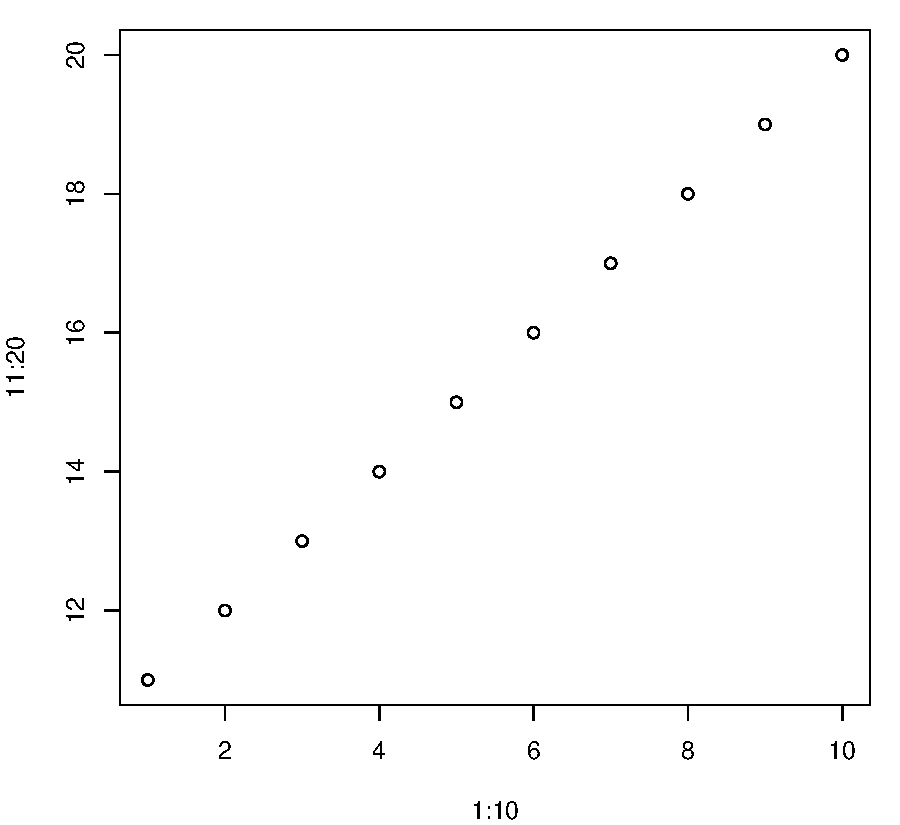
\includegraphics{articleTemplate-003}
\caption{CAPTION}
\end{center}
\end{figure}

\lipsum[2]
\begin{table}[H]
\caption{IR (\%) at CFRR= 100\% (SD) [number of classes]}
% latex table generated in R 3.0.2 by xtable 1.7-1 package
% Tue Apr 15 14:00:55 2014
\begin{table}[ht]
\centering
\begin{tabular}{rrr}
  \hline
 & V1 & V2 \\ 
  \hline
1 &   1 &  11 \\ 
  2 &   2 &  12 \\ 
  3 &   3 &  13 \\ 
  4 &   4 &  14 \\ 
  5 &   5 &  15 \\ 
  6 &   6 &  16 \\ 
  7 &   7 &  17 \\ 
  8 &   8 &  18 \\ 
  9 &   9 &  19 \\ 
  10 &  10 &  20 \\ 
   \hline
\end{tabular}
\end{table}
\end{table}


%\end{multicols}
%\setkeys{Gin}{width=1\textwidth}
\end{document}
